\documentclass[twocolumn,11pt]{article}
\setlength{\textheight}{9truein}
\setlength{\topmargin}{-0.9truein}
\setlength{\parindent}{0pt}
\setlength{\parskip}{10pt}
\setlength{\columnsep}{.4in}

\usepackage[utf8]{inputenc}
\usepackage{amsmath}
\usepackage{appendix}
\usepackage{graphicx}
\usepackage{multicol}
\usepackage{natbib}
\usepackage{url}

\title{Using an agent-based model to analyze usage of the Mosquito deterrence device in public parks}
\author{Clayton Pruitt}
\date{December 2019}

\graphicspath{{images/}}

\begin{document}
\pagestyle{plain}
 \twocolumn[
   \begin{@twocolumnfalse}
   \maketitle
   \setlength{\parindent}{0pt}
   \begin{abstract} Presbycusis is a condition that results in a loss of the ability to hear higher frequencies with age. The Mosquito is a sound deterrence device that uses high-frequency sounds to target youths from loitering in public parks.  In this paper we create an agent-based model to analyze the effectiveness of the device and to see whether the effects are relevant. We ultimately find that the Mosquito has a slight effect on the mean age of the park but no effect on the mode age, giving the impression that the device has little effect on the overall age distribution of the park's population. Thus, it appears that the Mosquito could potentially discriminate against youth. We conclude by suggesting further improvements for the model.
		\vspace{.3in} 
     \end{abstract}
    \end{@twocolumnfalse}]

\maketitle

\section*{Introduction}
There are times when groups considered undesirable are believed to make up a significant portion of the population of some environment. A simple example would be customers in a store after the store has closed. For such groups, deterrence methods are often used to discourage the undesirable group from remaining. For our example, an announcement over an intercom declaring that the store has closed could be used to encourage the customers to leave the store. 

In a recent article, Winberg (2019) describes a deterrence device referred to as a ``Mosquito" which uses high-pitched noises to irritate teenagers enough for them to leave public parks \citep{billypenn}. The United Kingdom distributor describes the Mosquito as a ``teenager repellent" and that it only affects people under the age of twenty-five years \citep{mosquitospecs}. This is possible through a condition known as prebyscusis, which is a common form of hearing loss that results in a loss of the ability to hear higher frequencies as age progresses \citep{prebyscusis}. There are concerns that the device discriminates against the youth as well as whether it accurately targets its specified age range, as prebyscusis does not have a one-to-one relation with age \citep{hearingthreshold}. In Philadelphia these concerns have led to a halt in further installation of Mosquito devices as well as an audit into whether the devices work at all \citep{billypenn}.

\begin{figure}[h]
    \centering
    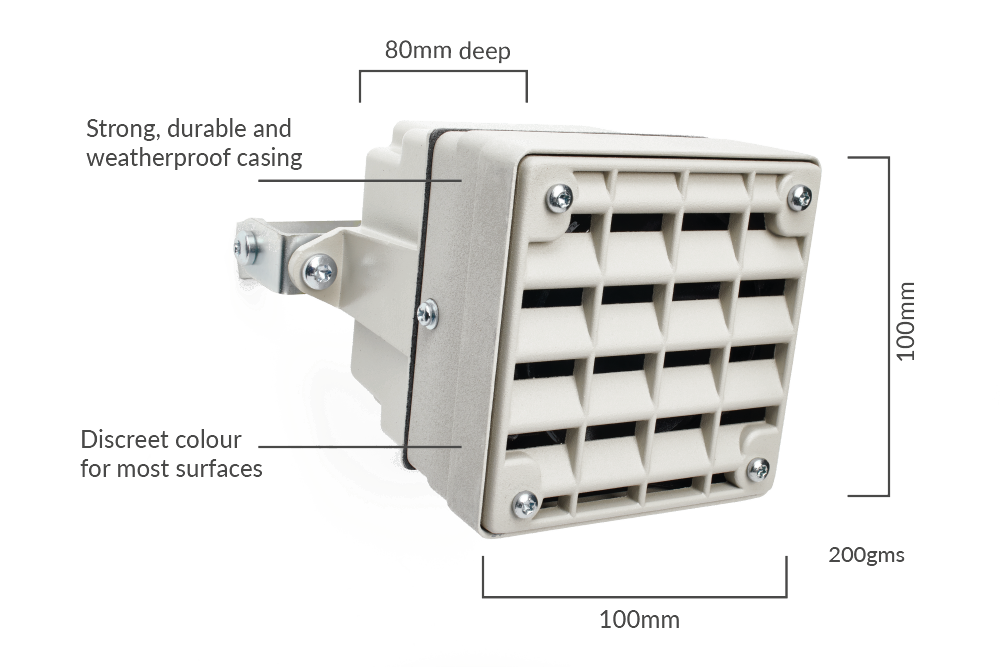
\includegraphics[width=1.0\columnwidth]{mosquito.png}
    \caption{The Mosquito device with labelled specifications \citep{mosquitoimage}.}
    \label{fig:mosquito}
\end{figure}


In this paper we explore the creation and usage of an agent-based model that can simulate the operation of the Mosquito deterrence device. Due to a lack of data on the Mosquito, we make generous assumptions on how it is used. However, the model is powerful and simple enough to use that tweaking of these assumptions can be made with minimal effort once appropriate data is available. Our model does not use any preexisting framework and is built from scratch using the Java object-oriented programming language. Microsoft Excel is used to generate input data and Python is used to analyze output data. We are looking to observe possible effects the Mosquito may have and find cases where analysis may prove more fruitful. The focus is not on proving real-world conjectures, but rather, showing that a simulated reality is enough to analyze the Mosquito and that integration with data as it becomes available will provide more meaningful results. The ultimate question we are seeking to answer is if the Mosquito could even have any effect at all.

\section*{Model}

\begin{figure*}[h]
    \centering
    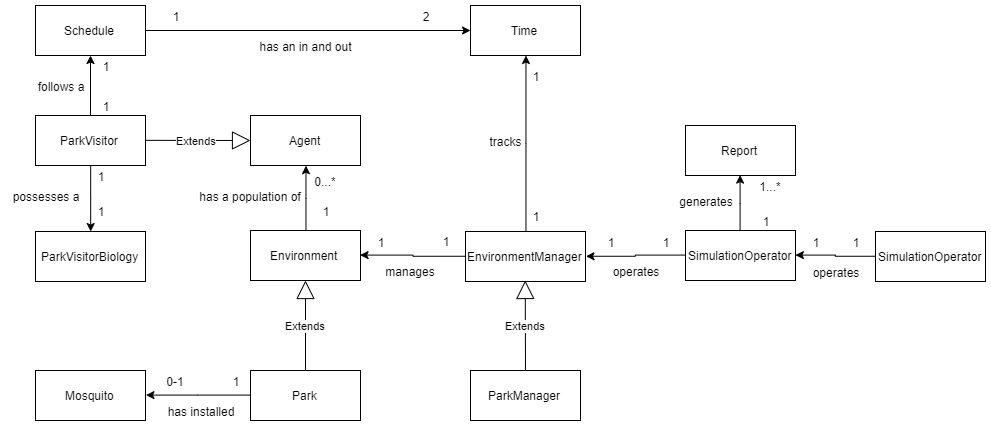
\includegraphics[width=1.0\textwidth]{umldomain.png}
    \caption{A UML domain model representing the agent-based model. The Agent, Environment, and EnvironmentManager objects are abstract and generalized by the ParkVisitor, Park, and ParkManager objects respectively. Arrows represent relations and the numbering represents how much are related. For example, a Park has zero to one Mosquitos and an Environment can have zero to infinitely many agents.}
    \label{fig:domain}
\end{figure*}

The overall structure of the model is visualized in Figure \ref{fig:domain} through a Unified Modeling Language (UML) domain model. There are thirteen objects contained in the model, three of which are abstract and generalized by other objects. Abstraction and generalizations were used so that the core of the model could be expanded on or re-purposed in future work. Relations and interactions between objects is kept at a minimum in order to maintain the ability to update and replace parts of the model with little effect on the rest of the model.

The Java programming language was used for implementation of the model, both for its ease-of-use and its adaptability. The core model is composed of the Agent, Environment, EnvironmentManager, Report, and Time objects. The Agent and Environment objects define base functionality that is expanded upon by the ParkVisitor and Park objects respectively. The EnvironmentManager object is defined as an interface; thus, its functionality is defined by the ParkManager object. The Time and Report objects are used as is without further functionality added by other objects. The remaining functionality of the model arises from the Mosquito, ParkVisitorBiology, and Schedule objects. The Mosquito contains the frequency it emits at and whether or not it is active. The ParkVisitorBiology defines the age of a ParkVisitor and the highest frequency an agent can hear. The Schedule object defines what time a ParkVisitor enters the Park and at what time they leave. From this point, if one of these objects is lower-cased it is to refer to them in the general, "real-world" sense. Otherwise, the object itself is being referred to with the exception of the Mosquito itself, which is always referred to as a proper noun.

Agents are generated using Excel spreadsheets. The model takes in a comma-separated value (.csv) file with fields for an Agent's name, age, time they enter the park, time they leave the park, and the highest frequency they can hear. This information is parsed and used to generate as many as agents as there are rows in the .csv file. The methods used to generate these agents are discussed in the following section.

The reality of the simulation is constrained within a hypothetical public park. Time progresses in continuous increments and loops from the end of one day to the next, though there is no distinction between different days. When an agent leaves the park, they are considered to be in a limbo state until they re-enter the park. Agents do not make decisions based off of the actions of other agents. The only stimulation for an agent is the Mosquito device itself. If an agent is able to hear the emitted frequency of the Mosquito they will immediately leave the park.

The simulation progresses through a series of cycles. Each cycle progresses the simulation by a consistent, pre-determined amount of time. At the beginning of a cycle a series of checks are made to determine whether the Mosquito should be active, whether there are any agents that should enter or leave the park according to their schedules, and whether or not any agents should leave the park due to the Mosquito. Each cycle will output a report after the final check.

A Report contains information corresponding to the point of simulated time it was generated. The information contained is the time of generation, the cycle, the park population, the mean age, and the mode age. The end of each cycle outputs a report containing a single row. This report is then added onto a cumulative report maintained by the SimulationOperator. The simulation is run twice, to generate one report for the park using the Mosquito and another report for the park not using the Mosquito. The two final reports are then outputted to .csv files by the model and analyzed with Python using the Matplotlib and NumPy libraries.

The parameters of the simulation are determined in an external configuration file. The file specifies the length of a cycle in minutes, the number of cycles run over the course of the simulation, the starting time of the simulation, the emitted frequency of the Mosquito, and the active hours of the Mosquito.

\section*{Methods}

One thousand agents were generated in total for the simulation. The normal distribution $N(\mu, \sigma^{2})$ was used for agent generation, where $\mu$ represents the mean of the distribution and $\sigma$ represents the standard deviation. The following assumptions were then made when generating agents:
\begin{enumerate}
    \item The age of the agents are normally distributed with $\mu = 45$, $\sigma = 10$, a minimum age of 0 (inclusive), and a maximum age of $100$ (exclusive). 
    \item The time an agent will visit a park is randomly generated from a normal distribution with $\mu = .70833$ days (i.e. 5:00PM) and $\sigma = .15$ days (i.e. $3.6$ hours).
    \item The time an agent will spend at the park is approximately linearly correlated with their age.
    \item The highest frequency an agent can hear exponentially decays with their age. 
\end{enumerate}

For the third assumption, the equation 
\begin{align*}
    f(x) = \frac{1}{24}(\frac{50}{11} - \frac{x}{22})
\end{align*} 
is used, where the parameter $x$ is the agent's age in years and the output is the time spent at the park in hours. The equation is a line and is derived from two further assumptions that a twelve-year old agent will spend $4$ hours at the park and a one-hundred year old agent will spend $0$ hours at the park. For generation, the agent's age had a random value between $-5$ and $5$ years added before being inputted into the function. 

For the fourth assumption, the equation 
\begin{align*}
    f(x) = 1000e^{-0.025 (x - 110)} + 8
\end{align*} is used, where the parameter $x$ is the agent's age in years and the output is the highest frequency the agent can hear in hertz. The equation was derived from the form 
\begin{align*}
    f(x) = me^{-a(x+b)}+c    
\end{align*}
and the values $a$, $b$, and $c$ were chosen so that an eighteen-year old agent can hear approximately up to $17.4$ kilohertz, a thirty-year old agent can hear up to approximately $15$ kilohertz, and the function can possess an asymptote at $8.0$ kilohertz. These values were motivated by a 2014 study on high-frequency hearing thresholds \citep{hearingthreshold}. The value for $m$ was chosen as $1000$ to convert from kilohertz to hertz. Similar to the third assumption, the agent's age had a random value between $-10$ and $10$ years added before being inputted into the function.

The simulation was configured to begin at 12:00PM with each cycle lasting for fifteen minutes. There were $96$ cycles run in total so that an entire day was simulated. The Mosquito was set to emit at a frequency of $17500$Hz with an activation time of 8:00PM and a deactivation time of 4:00AM.

As previously discussed, the only external stimuli that the agents react to is the Mosquito itself. Thus, an agent will only leave the park if they are scheduled to leave or if they cannot tolerate the Mosquito. It is assumed that the Mosquito will not deter the agent from visiting the park in the future.

\section*{Results}

\begin{figure*}[t!]
    \centering
    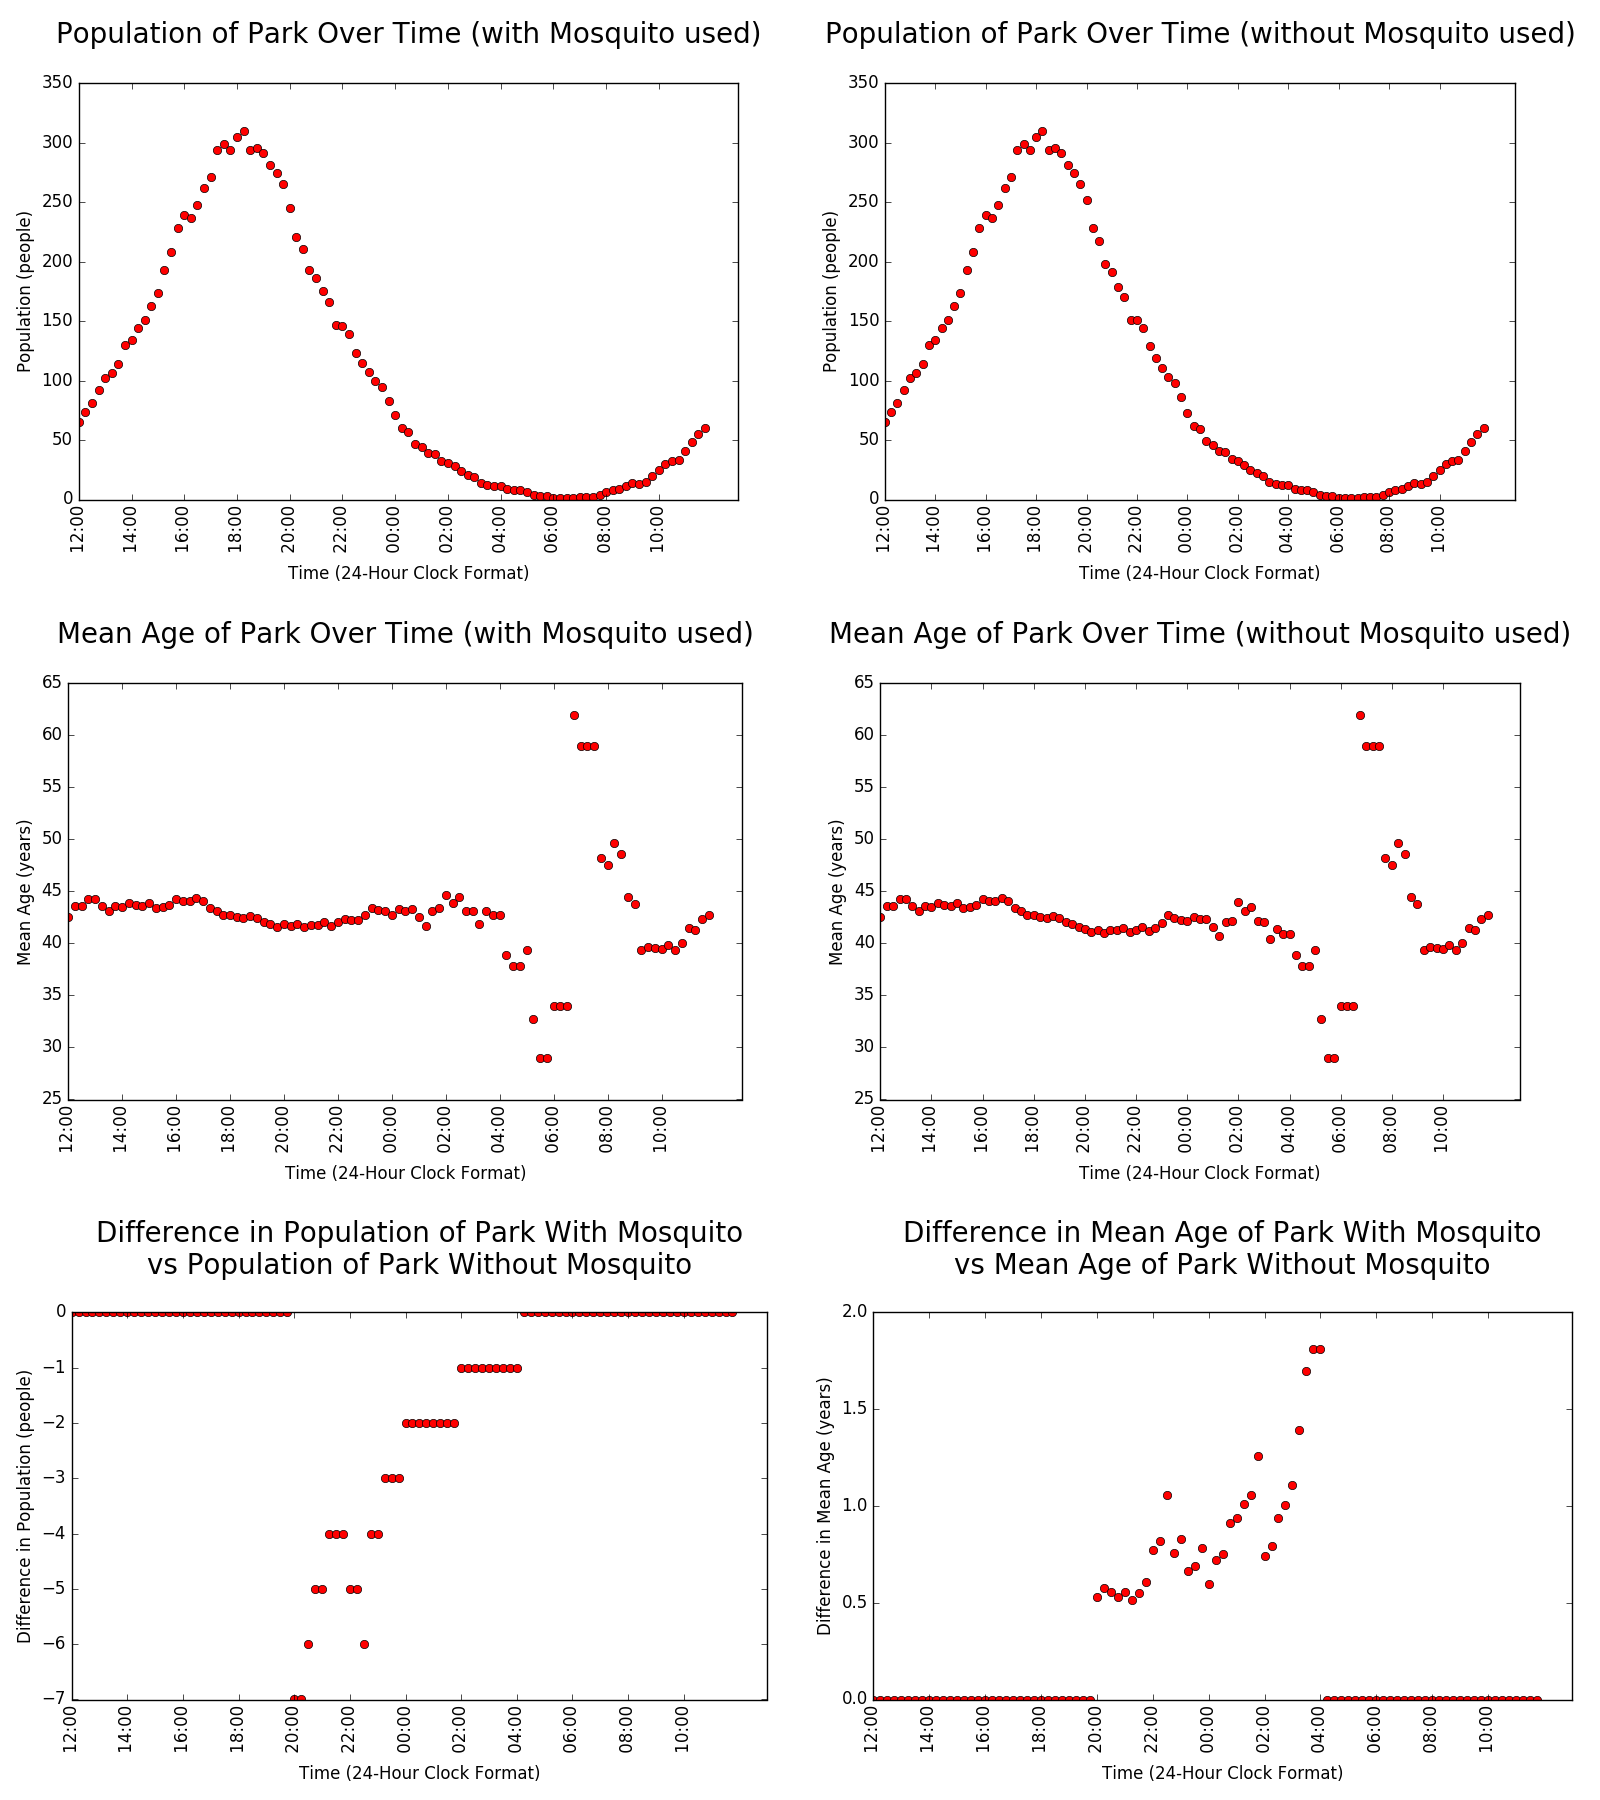
\includegraphics[width=0.75\textwidth]{results.png}
    \caption{The final results of the simulation which compare the differences of the park using or not using the Mosquito. The park using the Mosquito experiences a max loss of $7$ agents from its total population and an increase of about $2$ years in its mean age.}
    \label{fig:results}
\end{figure*}

The results of the simulation are summarized in Figure \ref{fig:results}. Areas of interest observed were 
\begin{enumerate}
    \item The population of the park with and without the Mosquito over time.
    \item The mean age of the park with and without the Mosquito over time.
    \item The difference in the population of the park with the Mosquito versus without the Mosquito over time.
    \item The difference in the mean age of the park with the Mosquito versus without the Mosquito over time.
    \item The difference in mode age of the park with the Mosquito versus without the Mosquito over time.
\end{enumerate}
The population of the park was observed to be highest between 6:00PM and 8:00PM at a population count of just over $300$ agents and lowest between 6:00AM and 8:00AM with a population count just over $0$ agents. When the park utilized the Mosquito, the population decreased by a maximum of $7$ agents and a minimum of $1$ agents between the Mosquito's active hours of 8:00PM and 4:00AM. Additionally, the park's mean age increased by a maximum of almost $2$ years between the Mosquito's active hours. The change in mode age is not represented in Figure \ref{fig:results} as it was found that the mode age did not change at all during the Mosquito's active hours.

\section*{Conclusion}
In this paper the effects of the Mosquito sound deterrence device were observed using an agent-based model to hypothesize the efficiency of the device. An agent-based model allowed for the effects to be observed on large populations, a task difficult in reality due to a lack of data. The model was created with Java and Excel and the results were analyzed using Python. Overall, the Mosquito does appear to be at least partially effective against youths, resulting in a small increase in the mean age of the park over the Mosquito's activation period. However, this effectiveness is minimal, as reflected by the lack of change in the mode age of the park. With the small increase in the mean age and a lack of change in the mode age, it appears that the Mosquito's effectiveness is not significant enough to affect the park's overall age distribution.

The model still bears room for improvement. Possible future implementations include a different means of generation for agents that does not resemble a normal distribution, agents possessing an aversion to visiting the park that is affected by exposure to the Mosquito, and running the simulation over multiple days instead of one. With these improvements, a more meaningful analysis could be made as the current analysis is dependent on multiple vague assumptions. However, the model as is still provides meaningful enough results.

\bibliographystyle{apalike}
\bibliography{references}

\appendix
\appendixpage
\section{GitHub}
The GitHub repository for the source code of the model can be found at https://github.com/clay10pruitt/mosquito-model.

\end{document}